%   PACKAGES AND CUSTOMIzATIONS  %%%%%%%%%%%%%%%%%%%%%%%%
\documentclass[12pt]{article}
\usepackage{amsmath}
\usepackage{amssymb}
\usepackage{amsthm}
\usepackage[pdfborder={0 0 0}]{hyperref}
\usepackage{graphicx}
\usepackage{caption}
\usepackage{natbib}
\usepackage{wrapfig}
\usepackage{enumitem}
\setlist[enumerate]{itemsep=0mm}
\usepackage{multirow}
\usepackage{lscape}
\usepackage{caption}
\usepackage{subcaption}
\usepackage{float}
\usepackage{hyperref}
\usepackage{tabularx}
\usepackage{rotating}
\captionsetup[subfigure]{position=top, labelfont=bf,textfont=normalfont,singlelinecheck=off,justification=raggedright}
\renewcommand{\vector}[1]{\mathbf{#1}}
\usepackage{adjustbox}
\usepackage{bm}


\newcommand{\transectAbb}{Data for each glacier are divided into lower hourglass (LH), lower circle (LC), lower midline (LM), upper hourglass (UH), upper circle (UC), upper midline (UM), and upper transect (UT).}
\newcommand{\params}{Topographic parameters are distance from centreline ($d_C$), elevation ($z$), aspect ($\alpha$), slope ($m$), northness ($N$), curvature ($\kappa$), and Sx. }
\newcommand{\boxplot}{Within each box, the mean is shown as a circle, the median as a horizontal line, the interquartile range (IQR) as a coloured box, two times the IQR as dashed lines beyond the box, and outliers as single points. }
\newcommand{\boxMatlab}{Red line indicates median, blue box shows first quantiles, bars indicate minimum and maximum values (excluding outliers), and red crosses show outliers, which are defined as being outside of the range of 1.5 times the quartiles (approximately $\pm2.7\sigma$). }
\newcommand{\topomap}{Arrows indicate glacier flow direction and black dots show snow depth sampling locations. }
\newcommand{\blackdots}{Observed SWE values are overlain on the maps. }


\begin{document}

back ground on Specific package
setting lower limit 

Final R2 value and rmse comparison of kriged, BMA, RK -> all density options?
sweKRIG vs SWE
sweRK vs SWE


Appendix -> manual for kriging 


%% Next time
- plot R2, rmse, residuals hist for RK
- discuss RK R2


\section{Kriging}

\subsection{Background}

Many physical surfaces vary continuously, and must therefore be spatially correlated, but at large distances the surface is statistically independent \citep{Davis1986}. If sampling point are distributed throughout the surface, the degree of spatial correlation can be determined and the surface can then be interpolated between the sampling points. Kriging is a geostatistical interpolation method that finds a set of optimal weights for the values at each sampling location based on the spatial correlation of measured values and then estimates values at unsampled locations \citep{Davis1986, Li2014}. The kriging estimates ($\hat{z}$) are found using the equation
\begin{equation}
\label{eq:kriging}
\hat{z}(x_0) - \mu = \sum_{i=1}^{n} \lambda_i [z(x_i)-\mu(x_0)],
\end{equation}
where $\mu$ is a known stationary mean, $\lambda_i$ is a kriging weight, $z(x_i)$ is the measured value of the surface at point $x_i$, $n$ is the number of sampled points used to make the estimation (depends on size of sampling window), and $\mu(x_0)$ is the mean of sampled in the search window \cite{Wackernagel2003, Li2008}. Slight variations on Equation \ref{eq:kriging} result in the various forms of kriging. The kriging weights are estimated by minimizing the variance, which is given by
\begin{align}
\mathrm{var}[\hat{z}(x_0)] &= E[(\hat{z}(x_0)-z(x_0)^2)]\\
&=\sum_{i=1}^{n}\sum_{j=1}^{n}\lambda_i \lambda_j C(x_i-x_j)+C(x_0-x_0)-2 \sum_{i=1}^{n} \lambda_i C(x_i-x_0),
\end{align}
where $C(x_i-x_j) = \mathrm{Cov}[z(x_i),z(x_j)]$ is the covariance of the surface \citep{Li2008}. Kriging assumes that the variance does not depend on the sample location and only depends on distance between samples (isotropic variance).  Anisotropic kriging allows for variance to change with direction. Isotropic variance was assumed in this study.

The surface is usually assumed to be noisy and this noise is captured by a ``nugget'' parameter that allows for the surface to not directly pass through each measured point (vary smoothly). The nugget is a residual that encompasses sampling-error variance as well as the spatial variance at distances less than the minimum sample spacing \citep{Li2008}. Spatial correlation of data is estimated using semivariance and is often plotted in the form of a semivariogram (see Section \ref{sec:variogram_intro}.  

There are many forms of kriging and each one is tailored to suit different data sets (see \cite{Li2014}). The two most appropriate types of kriging for this study are simple kriging and regression kriging. 

\subsubsection{Simple Kriging}

Simple kriging is used to estimate residuals about a constant and stationary mean $\mu$, which is typically calculated as the average of the data. Kriged estimates for simple kriging are found by slightly modifying Equation \ref{eq:kriging} to 
\begin{equation}
\hat{z}(x_0) = \sum_{i=1}^{n} \lambda_i z(x_i) +\left[1-\sum_{i=1}^{n} \lambda_i \right]\mu.
\end{equation}
Larger values of $\left[1-\sum_{i=1}^{n} \lambda_i \right]$ result in estimates that are closer to the data mean \citep{Li2008}. The value of $\left[1-\sum_{i=1}^{n} \lambda_i \right]$ generally increases in poorly sampled areas. 

\subsubsection{Regression Kriging}

Regression kriging estimates values between measurement locations by combining a regression estimate (see Section \ref{sec:linearregression}) with a kriged estimate of the regression residuals \citep{Hengl2007}. The regression estimate is determined using auxiliary variables (e.g. terrain parameters such as elevation and slope) and then simple kriging is used to fit the variation that was not explained by the regression and the assumed mean is 0 for the residuals. The two estimates of the surface are then added. The final estimate can be written as 
\begin{align}
\hat{z}(x_0) &= \hat{m}(x_0) + \hat{e}(x_0)\\
& = \sum^p_{k=0}\hat{\beta}_k \cdot	q_k(x_0)+ \sum_{i=1}^{n} \lambda_i \cdot e(x_i),
\end{align}
where $\hat{m}(x_0)$ is the regression estimate, $\hat{e}(x_0)$ is the interpolated residual, $\hat{\beta}_k$ are the estimated regression coefficients, $\lambda_i$ are the kriging weights for the residuals, and $e(x_i)$ is the residual at $x_i$.

Regression kriging can be thought of as an intermediate between pure kriging (no regression) and pure regression (high correlation) and can be more strongly skewed to either end-member based on the strength of the regression correlation. Regression kriging is mathematically equivalent to universal kriging, in which auxiliary variables are used directly to determine the kriging weights \citep{Hengl2007}. However, separating the trend analysis and kriging steps has the advantage of being able to test various regression methods beyond a basic linear trend. Kriging combined with regression has been found to produce better estimates of spatial fields when compared to simple kriging and co-kriging \citep{Knotters1995}.

\subsection{Methods}

\subsection{Results}

\subsubsection{Simple Kriging}

The interpolated snow accumulation patterns found using simple kriging are different for the three study glaciers  (Figure \ref{fig:sweKRIGING}). The lower half of Glacier 4 has a relatively even SWE, while the accumulation area has both low and high values of SWE. Glacier 2 has two distinct and relatively uniform areas --- the lower ablation area has low SWE ($\sim$ 0.1 m w.e.) and the upper ablation and accumulation areas have higher SWE values ($\sim$ 0.6 m w.e.). Glacier 13 does not appear to have any strong patterns and accumulation is generally low ($\sim$ 0.1--0.5 m w.e.). 

The mean SWE on each glacier found using simple kriging is considerably different to that found using a regression (Figure \ref{fig:BMSmodelledSWE}). Accumulation on Glacier 4 is higher and has larger spatially gradients in SWE when simple kriging is used. Conversely, simple kriging estimates are lower and have a smaller range for Glaciers 2 and 13.  The accumulation distribution estimated by simple kriging and by regression is qualitatively similar for Glacier 13 but differs considerably for Glacier 4 and 2. Glacier 4 has large SWE values in the accumulation area when simple kriging is used, which contrasts strongly with the mostly uniform accumulation estimated with regression. The converse is observed on Glacier 2, where the simple kriging estimate has a small SWE range and two distinct regions of SWE values while the regression estimate has a large range and a significant elevation gradient in accumulation.

Estimates of the nugget found using maximum likelihood in the DiceKriging package also vary between glaciers (Table \ref{tab:sweKrigNugget}). Nugget values are small for both Glacier 2 and 13 ($\sim$ 0.004 m w.e.) and do not vary when different density options are used. The nugget values for Glacier 4 are an order of magnitude larger and vary by $\sim$80\% of the minimum value. 

\begin{figure}
	\centering
	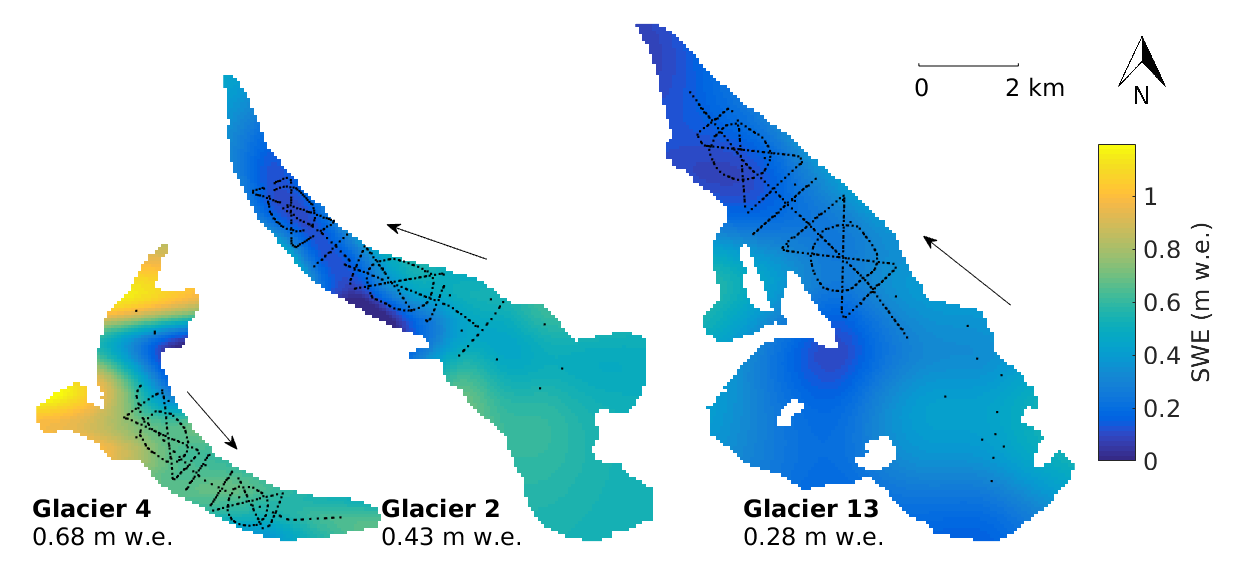
\includegraphics[width = \textwidth]{sweKriged.png}\\
	\caption{Estimated SWE found by kriging measured SWE. \topomap}
	\label{fig:sweKRIGING}
\end{figure}


\begin{table}[]
\centering
\caption{Nugget (m w.e.) estimated for SWE data using maximum likelihood in DiceKriging package.}
\label{tab:sweKrigNugget}
\begin{tabular}{c|ccc}
\textbf{\begin{tabular}[c]{@{}c@{}}Density\\ Option\end{tabular}} & \textbf{Glacier 4} & \textbf{Glacier 2} & \textbf{Glacier 13} \\ \hline
\textbf{S1} & 0.015 & 0.004 & 0.004 \\
\textbf{F1} & 0.013 & 0.003 & 0.003 \\ \hline
\textbf{S2} & 0.009 & 0.004 & 0.004 \\
\textbf{F2} & 0.009 & 0.003 & 0.003 \\ \hline
\textbf{S3} & 0.016 & 0.004 & 0.005 \\
\textbf{F3} & 0.017 & 0.002 & 0.003 \\ \hline
\textbf{S4} & 0.014 & 0.004 & 0.004 \\
\textbf{F4} & 0.009 & 0.002 & 0.003
\end{tabular}
\end{table}

\subsubsection{Residual Kriging}

The estimated distribution of regression residuals found using simple kriging varies between the three study glaciers (Figure \ref{fig:residualsKRIGING}). Generally, the range of residual values is highest on Glacier 4 and lowest on Glacier 13. Extreme value are located in the accumulation area of Glacier 4 with both strongly negative and strong positive residuals located within a kilometre of each other. Residuals show less variation on Glacier 2, although large negative residuals are present on the left side of the upper ablation area, close to the ice fall. Glacier 13 has the smallest range of residuals but the values are close to that of estimated SWE. The mean value of distributed residuals is positive for Glacier 4, indicating that the regression may have underestimated the total winter balance. Conversely, the mean residual for Glacier 2 is negative, indicating that the regression may have over estimated the total winter balance for this glacier. 

The winter balance found using regression kriging (Figure \ref{fig:Regression-Kriging}) shows a gradient in accumulation across the mountain range. Glacier 4 has the high mean SWE and Glacier 13 has the lowest mean SWE. All three glacier have the largest values of SWE in the upper part of the accumulation areas. 

The winter balance estimated using regression kriging is similar to the winter balance estimated using regressions for Glaciers 2 and 13 (Figure \ref{fig:Regression-Kriging}). The similarity is due to the relatively high explanatory power of the regressions, so the regression kriging estimate is closer to a pure regression. The distribution of accumulation on Glacier 4 is more strongly affected by the kriged residuals because the regression had low explanatory power, resulting in larger residual values that changed the snow distribution, particularly in the upper portion of the glacier. The regression kriging for Glacier 4 is therefore closer to pure kriging.

!!R2 for RK!!

\begin{figure}
	\centering
	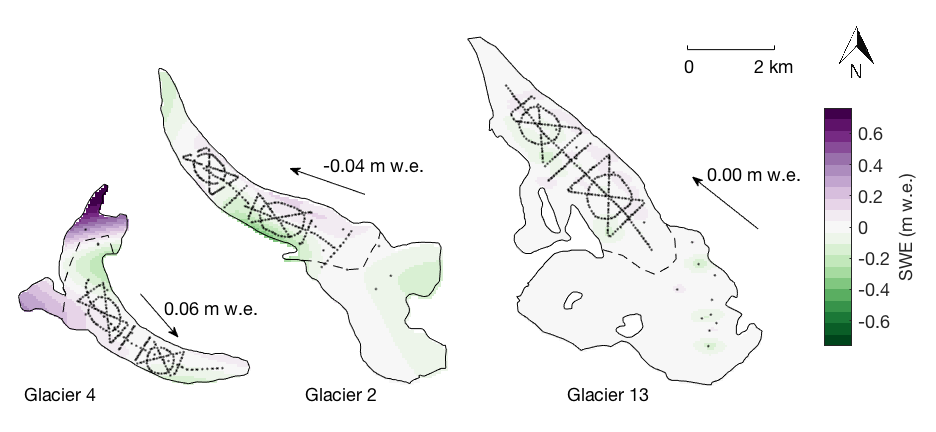
\includegraphics[width = \textwidth]{residualsKriged.png}\\
	\caption{Estimate of BMA residuals found by simple kriging. \topomap}
	\label{fig:residualsKRIGING}
\end{figure}

\begin{figure}
	\centering
	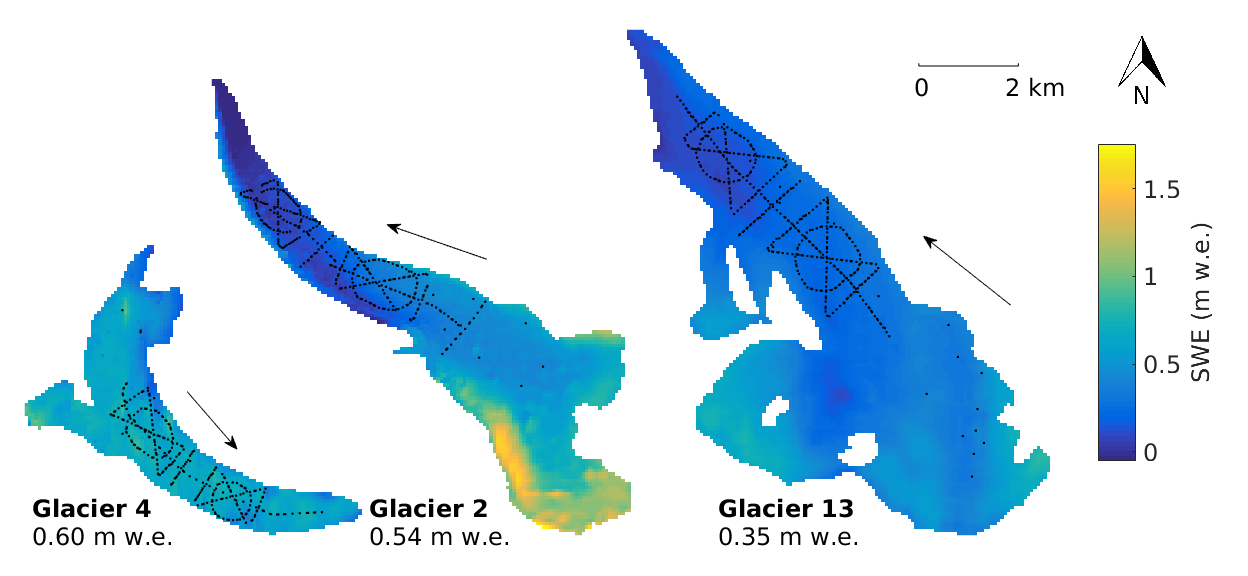
\includegraphics[width = \textwidth]{RegressionKriging.png}\\
	\caption{Estimated SWE found by adding the estimated residuals (simple kriging) to the estimated SWE found using BMA. \topomap}
	\label{fig:Regression-Kriging}
\end{figure}


\section{Kriging software}
\label{sec:KrigingMethods}
Data kriging was executed using the DiceKriging package in R (??). The function \texttt{KrigingR()} computes the kriged surface of input data through DiceKriging, as well as the upper and lower confidence intervals, the cross-validated (leave one out) estimates of SWE, as well as parameters that describe the kriging model fit (nugget, maximum log likelihood and mean constant). 

\bibliography{/home/glaciology1/Documents/MastersDocuments/MastersLit}
\bibliographystyle{igs}

\end{document} 